\documentclass[12pt]{ctexart}
\usepackage[a4paper, margin=2.5cm]{geometry}
\usepackage{setspace}
\usepackage{graphicx}
\usepackage{amsmath}
\usepackage{hyperref}

\setstretch{1.5}

\title{语义分析实验报告}
\author{程宣赫 \quad 2023202250}
\date{\today}

\begin{document}

\maketitle

\section{实验思路}

\subsection{整体任务框架分析}

本次实验是在已经完成词法分析和语法分析的基础上，进一步将源程序翻译为可被 LLVM 工具链处理的中间表示。语法分析阶段的主要目标是判断输入程序是否符合 SysY 语言的文法规则，并按照产生式的归约关系识别出程序中的声明、语句、表达式、函数定义等结构；而语义分析与中间代码生成阶段则需要在这些语法结构之上继续回答“这个结构表示什么”以及“它应当被翻译成什么样的目标形式”两个问题。因此，本实验的核心并不是重新识别语法，而是在语法归约过程中为不同非终结符附加语义属性，并根据这些属性生成等价的 LLVM IR。

从逻辑上看，语法分析到语义分析的过渡可以理解为从“结构识别”到“含义维护”的过渡。语法分析能够识别出一个表达式由哪些子表达式和运算符组成，但它本身并不直接说明该表达式的值保存在哪里、是否需要从内存中读取、是否可以在编译期求值，也不说明生成代码时需要使用哪条 LLVM 指令。为了解决这些问题，需要为语法成分设计能够传递信息的语义值。例如，表达式可以携带当前计算结果对应的立即数或虚拟寄存器；左值可以携带其内存地址；条件表达式可以携带用于控制流跳转的条件结构；数组声明可以携带维度信息；函数实参和形参则可以携带参数列表信息。这样，较小语法单元在归约为较大语法单元时，语义信息也可以同步向上传递。

在 LLVM IR 的生成过程中，另一个重要思想是将源语言中的高级结构逐步降解为更基础的 IR 操作。SysY 中的变量、赋值、表达式、函数调用、条件分支和循环语句，在 LLVM IR 中分别需要映射为 \texttt{alloca}、\texttt{load}、\texttt{store}、算术指令、比较指令、\texttt{call}、\texttt{br} 和 \texttt{ret} 等低级指令。源程序中的变量名不能直接作为计算结果使用，而需要先通过符号信息找到对应地址，再根据上下文决定是否生成 \texttt{load} 指令。类似地，源程序中的 \texttt{if} 和 \texttt{while} 并不是 LLVM IR 的单条高级指令，而需要被拆分为若干基本块以及基本块之间的条件或无条件跳转。因此，本实验需要在语义分析阶段同时维护数值语义和控制流语义。

此外，LLVM IR 采用静态单赋值思想，每个虚拟寄存器只能被定义一次。虽然本实验没有实现完整的 SSA 构造和优化过程，但在直接生成文本形式 IR 时仍然需要保证每次中间计算都使用新的虚拟寄存器名称，并且每个基本块以合法的终结指令结束。基于这一要求，实验中需要统一管理寄存器编号、标签编号和当前基本块是否已经结束等状态。这样既能避免重复定义寄存器，也能避免在已经出现 \texttt{return}、\texttt{break} 或跳转之后继续向同一基本块追加不合法指令。

总体而言，本实验的理论框架可以概括为：词法分析首先将源程序转换为记号流，语法分析按照文法规则完成结构识别，语义动作在归约过程中维护符号、类型、值和控制流等信息，最终将 SysY 程序中的高级语言结构翻译为符合 LLVM IR 语法和语义约束的中间代码。这个过程体现了编译器前端从“识别程序”到“理解程序并生成中间表示”的完整过渡。

\subsection{整体执行流程与功能划分}

从实现层面看，本实验的核心是为不同归约规则设计语义动作。每类语义动作都对应一个明确的翻译问题：声明类动作需要建立名字与存储位置的关系，表达式类动作需要产生可继续传递的语义值，赋值和数组访问需要区分左值地址与右值内容，函数相关动作需要处理函数边界与参数传递，控制流动作则需要把高级语句转换成标签和跳转。也就是说，本实验不是先凭空设计所有结构体，而是在逐类实现语义动作时，根据“后续生成 LLVM IR 还缺少什么信息”逐步引入 \texttt{Symbol}、\texttt{Value}、\texttt{DimList}、\texttt{ArgList}、\texttt{ParamList}、\texttt{CondNode}、\texttt{IfContext} 和 \texttt{LoopContext} 等辅助结构。

\subsubsection{常量声明与常量表达式}

首先需要处理的是常量声明和常量表达式。对于 \texttt{const int a = 3;} 这样的语句，语义动作不仅要识别出这是一个常量定义，还要保存“标识符 \texttt{a} 对应的值是 \texttt{3}”这一信息，因为后续表达式中再次使用 \texttt{a} 时，应当能够直接得到它的常量值。因此，常量声明自然会引出符号表设计：在 \texttt{Symbol} 中保存常量名称、是否为常量的标记 \texttt{is\_const}、常量值 \texttt{const\_value}、是否为全局符号的标记 \texttt{is\_global}，以及当前作用域层级 \texttt{scope\_level}。

在归约到 \texttt{ConstDef} 时，右侧的初始化值会先被归约为一个常量语义值，随后根据当前是否处于函数内部采用不同处理方式。如果 \texttt{in\_function} 为假，说明该常量位于全局作用域，此时调用 \texttt{add\_global\_symbol()} 将其登记为全局常量，并输出 \texttt{@name = constant i32 value} 形式的 LLVM IR 定义；如果 \texttt{in\_function} 为真且不是数组常量，则调用 \texttt{add\_local\_const\_symbol()} 将其登记为局部常量，只在符号表中保存 \texttt{is\_const}、\texttt{const\_value} 和 \texttt{scope\_level}，不再为它生成额外的 \texttt{alloca} 或 \texttt{load}。这样既区分了全局常量和局部常量，也使局部常量能够随着 \texttt{push\_scope()} 与 \texttt{pop\_scope()} 正确进入和退出作用域。

后续如果在表达式中遇到常量标识符，\texttt{find\_symbol()} 会从符号表末尾向前查找，因此内层局部常量可以优先于外层同名符号被找到。随后 \texttt{lvalue\_from\_symbol()} 根据 \texttt{is\_const} 和 \texttt{const\_value} 直接返回 \texttt{new\_const\_value()}，避免像普通变量一样生成 \texttt{load} 指令。对于带维度的局部常量数组，当前实现将其作为局部数组处理，通过 \texttt{add\_local\_array\_symbol()} 分配数组空间；全局常量数组则仍由 \texttt{add\_global\_symbol()} 记录维度并输出全局数组定义。

常量表达式还涉及另一个问题：它的结果必须在编译过程中直接算出。例如 \texttt{const int a = 1 + 2 * 3;} 的右侧应在归约过程中得到 \texttt{7}，数组维度中的 \texttt{2 + 3} 也必须立即求出大小。因此，实验中引入了 \texttt{const\_eval\_mode} 标记当前是否处于常量求值模式，并通过 \texttt{ConstEvalBegin} 在进入常量表达式前临时打开该模式。在该模式下，\texttt{emit\_binary()} 和 \texttt{emit\_compare()} 不再输出普通 LLVM 指令，而是直接根据左右操作数的 \texttt{const\_value} 计算出新的 \texttt{Value}。对于数组维度，还需要通过 \texttt{DimList} 和 \texttt{append\_dim()} 保存计算得到的维度大小，使后续数组声明能够得到确定的存储空间规模。

\subsubsection{变量声明、数组声明与初始化}

变量声明首先要解决的是“变量名对应什么存储位置”的问题。源程序中写的是 \texttt{int a;} 或 \texttt{a = 1;}，但 LLVM IR 中后续读写变量时必须知道它对应的地址。因此，变量声明和常量声明一样需要依赖符号表；不同的是，变量的值会在运行时发生变化，符号表中不能只保存当前值，而应保存变量的存储位置。后续赋值语句通过该地址生成 \texttt{store}，表达式读取时再通过该地址生成 \texttt{load}。

由于全局变量和局部变量在 LLVM IR 中的存储方式不同，变量声明还必须区分作用域。如果当前不在函数内部，即 \texttt{in\_function} 为假，则变量属于全局作用域，实验通过 \texttt{add\_global\_symbol()} 输出 \texttt{@name = global i32 init} 形式的全局定义，并在 \texttt{Symbol} 中记录 \texttt{is\_global=1}、变量名、全局符号地址和初始值。全局变量的初始化值需要在定义处确定，因此带初始化的全局变量会把 \texttt{InitVal} 的常量值直接写入全局定义；没有显式初始化时则使用 \texttt{0}。

如果当前处于函数内部，普通局部变量通过 \texttt{add\_local\_symbol()} 处理。该函数会先检查当前 \texttt{scope\_level} 下是否已经存在同名局部符号，随后使用 \texttt{new\_reg()} 生成一个新的 LLVM 虚拟寄存器，并输出 \texttt{alloca i32} 为该变量分配局部存储空间。符号表中保存的 \texttt{ptr} 不是变量当前的整数值，而是这块局部存储空间的地址。对于带初始化的局部变量，语义动作会先取得这个地址，再调用 \texttt{emit\_store()} 将右侧表达式的值写入该地址，从而完成运行时初始化。

数组声明还涉及额外的问题：除了知道数组名对应的基地址，还必须知道数组的维度和总大小，才能分配空间并在后续访问元素时计算偏移。因此实验中使用 \texttt{DimList} 保存数组维度，并通过 \texttt{append\_dim()} 在归约 \texttt{VarArrayDims} 时逐步记录每一维大小。全局数组由 \texttt{add\_global\_symbol()} 输出 \texttt{zeroinitializer} 形式的全局数组定义；局部数组由 \texttt{add\_local\_array\_symbol()} 先输出 \texttt{alloca [N x i32]} 分配连续空间，再通过 \texttt{bitcast} 转换为便于后续 \texttt{getelementptr} 寻址的 \texttt{i32*} 基地址。这样，变量和数组声明最终都被统一记录到符号表中，为后续左值表达式、赋值语句和数组元素访问提供地址信息。

\subsubsection{表达式计算与语义值传递}

声明部分建立了符号表之后，表达式计算需要解决的是“每个表达式归约后向上层传递什么信息”。如果只传递一个字符串，就无法区分 \texttt{3} 这样的立即数、\texttt{\%r1} 这样的计算结果，以及变量 \texttt{a} 对应的地址。LLVM IR 对这三类信息的处理方式不同：立即数可以直接作为操作数，计算结果通常已经保存在虚拟寄存器中，而地址必须先通过 \texttt{load} 取出内容后才能参与运算。因此，表达式计算自然需要一个统一的语义值结构。

为此实验中设计了 \texttt{Value}。其中，\texttt{text} 保存当前表达式可在 IR 中使用的文本形式，\texttt{ptr} 保存左值对应的地址，\texttt{is\_lvalue} 用于说明当前表达式是否表示地址，\texttt{is\_const} 与 \texttt{const\_value} 用于常量求值。对于整数常量，使用 \texttt{new\_const\_value()} 构造常量语义值；对于普通运算得到的寄存器结果，使用 \texttt{new\_value()} 保存寄存器名；对于变量或数组元素这样的左值，使用 \texttt{new\_lvalue()} 保存其地址。这样，每条表达式产生式都可以把自身结果封装为 \texttt{Value} 继续向上传递。

表达式计算还需要解决“什么时候读取地址中的值”的问题。为此实验中封装了 \texttt{value\_as\_rvalue()}：如果传入的是立即数或寄存器结果，则直接返回其文本形式；如果传入的是左值地址，则调用 \texttt{new\_reg()} 生成新寄存器，并输出 \texttt{load i32, i32* ...} 将地址中的值读出。这样，上层语义动作在处理加减乘除、比较、函数实参等需要右值的场景时，不必重复判断左值和右值，只需统一调用该函数即可。

在具体运算中，算术表达式通过 \texttt{emit\_binary()} 生成 \texttt{add}、\texttt{sub}、\texttt{mul}、\texttt{sdiv} 和 \texttt{srem} 等指令，并将结果寄存器重新封装为 \texttt{Value}。比较表达式通过 \texttt{emit\_compare()} 生成 \texttt{icmp} 得到 \texttt{i1} 结果，再用 \texttt{zext} 扩展为 \texttt{i32}，从而与 SysY 中整数表达式的使用方式保持一致。如果当前处于 \texttt{const\_eval\_mode}，这些函数则不输出运行时指令，而是直接计算并返回常量 \texttt{Value}。因此，表达式部分的整体工作流就是：子表达式先给出语义值，当前规则根据运算符生成常量结果或 IR 指令，再把新的语义值传给更高层。

\subsubsection{左值表达式、赋值与数组寻址}

左值表达式要解决的是“同一个标识符在不同上下文中到底表示地址还是值”的问题。例如 \texttt{a=1} 中的 \texttt{a} 位于赋值左侧，需要作为 \texttt{store} 的目标地址；而 \texttt{b=a+1} 中的 \texttt{a} 位于表达式内部，需要先从地址中 \texttt{load} 出当前值。为了让这两种使用方式不混淆，实验中将 \texttt{LVal} 的基本语义设计为“位置”，即优先返回左值地址，而是否读取地址中的内容交给上层表达式或语句决定。

在归约 \texttt{LVal} 时，语义动作首先通过 \texttt{find\_symbol()} 查找标识符。如果没有找到，就调用 \texttt{semantic\_error()} 报告未定义符号；如果找到，则调用 \texttt{lvalue\_from\_symbol()} 构造对应语义值。对于普通变量，该函数返回包含变量地址的左值 \texttt{Value}；对于普通常量，由于其值已经保存在符号表中，因此直接返回 \texttt{new\_const\_value()}；对于数组元素，则需要根据数组基地址和下标列表进一步计算元素地址。

数组寻址需要解决“多维下标如何转为一维内存偏移”的问题。符号表中的 \texttt{dims} 和 \texttt{total\_size} 保存了数组维度信息；下标列表则通过 \texttt{LValIndexList} 归约并使用 \texttt{ArgList} 保存。对于全局数组，先用 \texttt{bitcast} 将全局数组指针转换为 \texttt{i32*} 基地址；对于局部数组，符号表中已经保存了 \texttt{bitcast} 后的基地址。随后，若是一维数组，偏移就是第一个下标；若是二维数组，则计算 \texttt{row * dims[1] + col}，最后通过 \texttt{getelementptr i32, i32* base, i32 offset} 得到目标元素地址，并将其作为左值返回。

赋值语句正好体现了左值与右值的分工。归约到 \texttt{LVal ASSIGN Exp} 时，左侧 \texttt{LVal} 保持为地址，右侧 \texttt{Exp} 通过 \texttt{value\_as\_rvalue()} 转换为可存储的整数值，最后调用 \texttt{emit\_store()} 输出 \texttt{store i32 value, i32* ptr}。因此，无论赋值目标是普通变量还是数组元素，都可以统一为“先得到目标地址，再把右值写入该地址”的流程。

\subsubsection{函数定义、参数处理、函数调用与返回}

函数相关语义动作需要解决的是“函数如何开始、参数如何进入函数体、调用如何产生结果、返回如何结束当前控制流”。LLVM IR 中的函数不是一个普通语句，而是由 \texttt{define} 头部、形参列表、入口基本块、函数体指令和 \texttt{ret} 指令组成。因此，在归约到函数头部时就必须输出函数定义并初始化函数内部状态，而不能等整个函数体归约完才处理。

为了处理形参，实验中使用 \texttt{ParamList} 保存形参名称。归约 \texttt{FuncFParams} 时通过 \texttt{append\_param()} 逐个收集参数；进入函数体前调用 \texttt{begin\_function()}。该函数根据返回类型输出 \texttt{define i32} 或 \texttt{define void}，将每个形参写成 LLVM 形参形式 \texttt{\%name\_p}，随后建立 \texttt{entry} 基本块。由于后续函数体中使用形参时仍希望像普通局部变量一样通过符号表查找地址，所以 \texttt{begin\_function()} 会为每个形参调用 \texttt{add\_local\_symbol()} 分配局部地址，再把传入的参数值 \texttt{store} 到该地址中。

函数开始时还需要重置函数内部状态。实验中在 \texttt{begin\_function()} 中设置当前返回类型、清空返回标记、设置 \texttt{in\_function}，调用 \texttt{reset\_function\_state()} 重置寄存器编号、标签编号和控制流栈，并通过 \texttt{push\_scope()} 建立函数作用域。函数结束时调用 \texttt{end\_function()}，如果函数体中没有显式 \texttt{return}，则根据返回类型补充 \texttt{ret i32 0} 或 \texttt{ret void}；随后不断 \texttt{pop\_scope()} 清理局部符号，并将 \texttt{in\_function} 置回假。

函数调用则需要先收集实参列表。实验中使用 \texttt{ArgList} 保存调用实参，归约 \texttt{FuncRParams} 时通过 \texttt{append\_arg()} 逐个追加表达式结果。真正生成调用时，\texttt{emit\_call()} 会把每个实参通过 \texttt{value\_as\_rvalue()} 转换为右值，并输出 \texttt{call i32 @name(...)}，调用返回值再封装为新的 \texttt{Value} 参与后续表达式。对于 \texttt{return} 语句，\texttt{emit\_return()} 根据当前函数返回类型输出 \texttt{ret i32 value} 或 \texttt{ret void}，同时设置 \texttt{function\_has\_return} 和 \texttt{current\_block\_terminated}。对于输入输出，实验将 \texttt{scanf} 和 \texttt{printf} 特判为运行时函数 \texttt{getint()} 和 \texttt{putint()}，并通过 \texttt{emit\_runtime\_decls()} 与 \texttt{runtime.c} 完成声明和链接。

\subsubsection{控制流语句与短路求值}

控制流语句要解决的是“程序下一步执行到哪里”的问题。LLVM IR 没有直接对应 SysY 中 \texttt{if}、\texttt{while}、\texttt{break} 和 \texttt{continue} 的高级语句，因此必须用基本块标签和 \texttt{br} 指令显式表示执行路径。为了能够不断生成新的基本块，实验中使用 \texttt{new\_label()} 统一分配标签，并通过 \texttt{emit\_label()} 输出基本块入口、通过 \texttt{emit\_br()} 输出无条件跳转。同时，\texttt{current\_block\_terminated} 用于记录当前基本块是否已经以 \texttt{return}、\texttt{break}、\texttt{continue} 或 \texttt{br} 结束，从而避免继续向已终止的基本块追加指令。

对于 \texttt{if/else}，需要保存 then 分支、else 分支和结束位置之间的关系，因此实验中设计了 \texttt{IfContext}。归约到 \texttt{IfHead} 时调用 \texttt{begin\_if\_unified()}，该函数创建 then、else 和 end 标签，并调用 \texttt{emit\_cond\_branch()} 根据条件跳转到 then 或 else；随后输出 then 标签并开始生成 then 分支代码。遇到 \texttt{ElseHead} 时，\texttt{switch\_to\_else()} 记录 then 分支是否已经终止，如果没有终止则补充到 end 的跳转，然后输出 else 标签。整个条件语句结束时，根据是否有 else 分支分别调用 \texttt{finish\_if\_without\_else()} 或 \texttt{finish\_if\_with\_else()}，补齐剩余跳转并输出 end 标签。由于 \texttt{IfContext} 以栈形式保存，嵌套 \texttt{if} 也可以正确匹配各自的标签。

对于 \texttt{while}，需要保存条件判断块、循环体块和循环退出块，因此实验中设计了 \texttt{LoopContext}。归约到 \texttt{WhileBegin} 时调用 \texttt{begin\_while()}，先创建 cond、body 和 end 标签，并跳转到条件块；条件归约完成后调用 \texttt{while\_condition()}，根据条件为真或假跳转到 body 或 end；循环体结束后调用 \texttt{end\_while()} 跳回 cond 标签并输出 end 标签。由于循环上下文同样以栈形式保存，\texttt{break} 可以通过 \texttt{emit\_break()} 跳转到当前最内层循环的 end 标签，\texttt{continue} 可以通过 \texttt{emit\_continue()} 跳转到当前最内层循环的 cond 标签。

逻辑表达式还涉及短路求值问题。对于 \texttt{\&\&}，左侧为假时右侧不应执行；对于 \texttt{||}，左侧为真时右侧不应执行。如果简单先计算左右两侧再做整数运算，就会破坏源语言语义。因此实验中设计 \texttt{CondNode} 保存条件表达式结构，其中普通条件是叶子节点，逻辑与和逻辑或是二叉节点。最终由 \texttt{emit\_cond\_branch()} 根据真标签和假标签递归生成跳转：逻辑与在左侧为真时才进入右侧判断，逻辑或在左侧为假时才进入右侧判断。这样，条件表达式不再只是产生一个普通值，而是直接服务于控制流跳转。

通过以上六类语义动作，程序在 \texttt{yyparse()} 的归约过程中逐步完成从 SysY 结构到 LLVM IR 的翻译。生成 \texttt{output.ll} 后，再通过脚本调用 \texttt{llc} 转换为汇编，并使用 \texttt{gcc} 与 \texttt{runtime.o} 链接生成可执行程序，最终形成从语义动作、IR 生成到程序运行验证的完整流程。

\section{实验中遇到的问题及解决方法}

\subsection{\texttt{if-else} 语句的移进规约冲突}

\subsubsection{问题解释}

实验中遇到的第一个主要问题是 \texttt{if-else} 语句的二义性，也就是常见的 dangling else 问题。最初的想法是沿用语法分析阶段中通过优先级处理冲突的方式，为不带 \texttt{else} 的 \texttt{if} 规则设置一个较低优先级，例如使用类似 \texttt{\%prec LOWER\_THAN\_ELSE} 的写法，让 \texttt{else} 优先和最近的 \texttt{if} 结合。这样在纯语法分析阶段可以较快消除移进规约冲突。

但是进入语义分析和 LLVM IR 生成阶段后，这种写法变得不够方便。原因在于 \texttt{if} 语句不再只是完成语法匹配，还需要在不同位置插入语义动作：识别到条件后要立即生成 then、else 和 end 标签，并输出条件跳转；进入 \texttt{else} 前要补充 then 分支到 end 的跳转；整个语句结束后还要根据是否存在 \texttt{else} 收束控制流。如果继续依赖优先级强行解决 dangling else，语法规则表面上较短，但语义动作需要插入在规则中间，和原来的优先级处理混在一起后很难维护，也容易再次触发移进规约冲突。

\subsubsection{解决方法}

为了解决这个问题，实验中放弃了单纯依赖优先级的方案，改为从文法结构上消除二义性。具体做法是将语句分为 \texttt{MatchedStmt} 和 \texttt{UnmatchedStmt} 两类：\texttt{MatchedStmt} 表示所有 \texttt{if} 都已经和对应的 \texttt{else} 匹配完成的语句；\texttt{UnmatchedStmt} 表示还存在尚未匹配 \texttt{else} 的 \texttt{if} 语句。这样，\texttt{else} 在文法层面自然会归属于最近的未匹配 \texttt{if}，不再需要额外依赖优先级规则。

在这一结构下，语义动作也更容易安排。遇到 \texttt{IfHead} 时调用 \texttt{begin\_if\_unified()} 生成条件跳转和 then 标签；遇到 \texttt{ElseHead} 时调用 \texttt{switch\_to\_else()} 切换到 else 分支；当归约为不带 \texttt{else} 的 \texttt{UnmatchedStmt} 时调用 \texttt{finish\_if\_without\_else()}；当归约为带 \texttt{else} 的完整匹配语句时调用 \texttt{finish\_if\_with\_else()}。通过这种 matched/unmatched 的拆分，既解决了移进规约冲突，也让控制流标签的生成位置更加清晰。

\subsection{逻辑表达式短路求值的处理}

\subsubsection{问题解释}

实验中遇到的第二个主要问题是逻辑表达式的短路求值。对于普通的算术表达式，例如 \texttt{a+b} 或 \texttt{x*y}，可以先分别计算左右两侧，再生成对应的二元运算指令。但逻辑与 \texttt{\&\&} 和逻辑或 \texttt{||} 不能简单按照这种方式处理，因为它们具有短路语义：对于 \texttt{A \&\& B}，如果 \texttt{A} 已经为假，那么 \texttt{B} 不应再被计算；对于 \texttt{A || B}，如果 \texttt{A} 已经为真，那么 \texttt{B} 也不应再被计算。

这个问题在语义分析和 IR 生成阶段会带来额外复杂性。首先，逻辑表达式不只是产生一个普通整数结果，它往往直接决定 \texttt{if} 或 \texttt{while} 应该跳转到哪个基本块。其次，右侧表达式中可能包含函数调用、赋值或数组访问等具有副作用的操作，如果无条件计算左右两侧，就可能改变源程序原本的执行语义。例如在 \texttt{a != 0 \&\& b / a > 1} 中，如果左侧为假，右侧除法本来不应执行；若直接计算两侧，就可能产生除零等错误。

\subsubsection{解决方法}

因此，完整解决短路求值需要把逻辑表达式和控制流生成结合起来处理，而不能只把 \texttt{\&\&} 和 \texttt{||} 当作普通二元运算。理想情况下，应当为条件表达式保存其逻辑结构，并在生成 IR 时根据真分支和假分支标签递归地产生跳转：逻辑与在左侧为真时才进入右侧判断，逻辑或在左侧为假时才进入右侧判断。

本次实验中暂时没有完整解决这一问题。当前实现的重点主要放在常量、变量、表达式、赋值、函数和基本控制流的翻译上，对于逻辑表达式短路求值仍可作为后续改进方向。后续如果继续完善，可以围绕条件表达式建立专门的数据结构来保存逻辑关系，并在 \texttt{if}、\texttt{while} 的条件跳转生成阶段统一展开短路控制流，从而保证逻辑表达式的执行顺序与源语言语义完全一致。

\section{实验结果}

本实验选取四个测试用例对编译结果进行验证。每个测试用例均先由编译器生成 \texttt{output.ll}，再通过 \texttt{llc} 生成汇编文件 \texttt{output.s}，最后使用 \texttt{gcc} 与运行时库 \texttt{runtime.o} 链接得到可执行文件 \texttt{program}。在得到可执行文件后，进一步运行 \texttt{program} 并记录其标准输入、标准输出和标准错误输出。四个测试均能够成功生成并运行可执行程序，运行结果如下所示。

\subsection{测试用例一}

测试用例一主要验证基本输入、加法表达式、赋值和输出语句。运行时输入为 \texttt{1 2}，程序输出为 \texttt{3}，说明变量读入、表达式计算和 \texttt{printf} 输出均能够正常工作。

\begin{figure}[htbp]
    \centering
    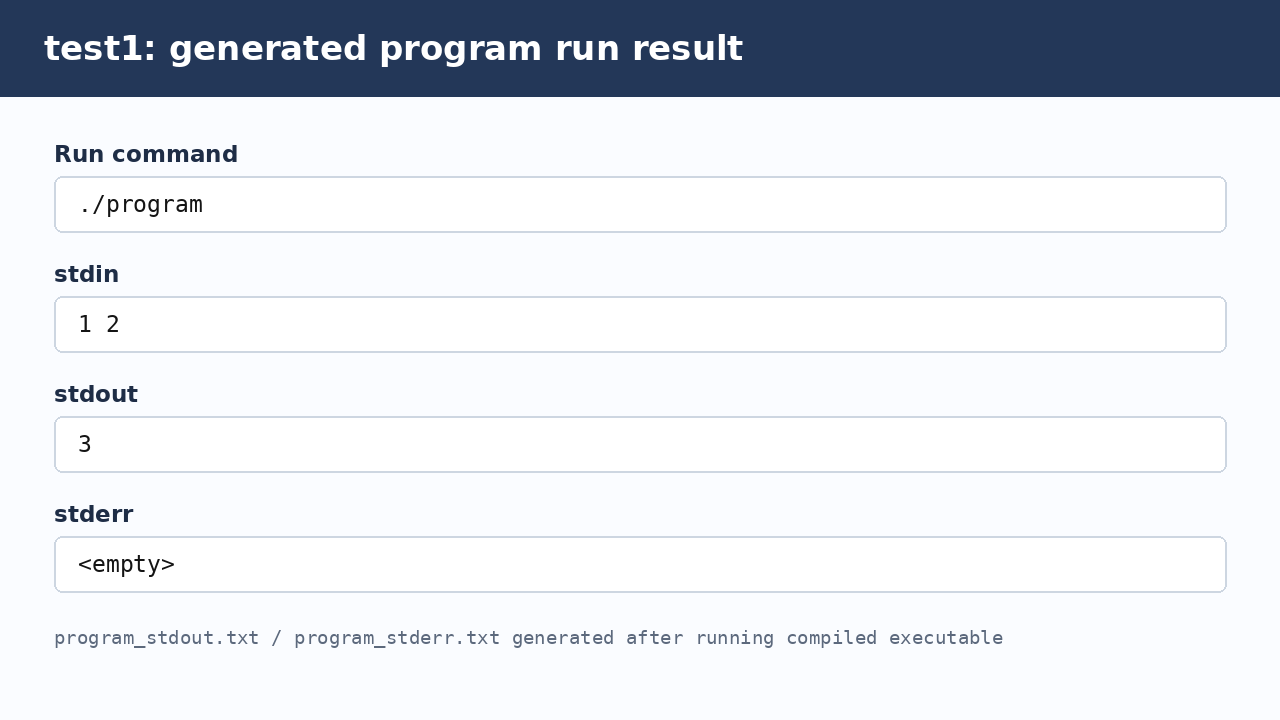
\includegraphics[width=0.95\textwidth]{output/test1/program_result.png}
    \caption{测试用例一运行结果}
\end{figure}

\subsection{测试用例二}

测试用例二覆盖函数递归调用、常量定义、二维数组访问、条件语句、循环语句以及 \texttt{break}/\texttt{continue} 等结构。运行时输入为 \texttt{99}，程序能够输出递归计算、条件分支、循环和数组访问相关结果。

\begin{figure}[htbp]
    \centering
    
\includegraphics[width=0.95\textwidth]{output/test2/program_result.png}
    \caption{测试用例二运行结果}
\end{figure}

\subsection{测试用例三}

测试用例三为多项式乘法程序，主要验证一维数组、嵌套循环、数组元素累加和多组输入输出。运行时输入为 \texttt{3 2 1 2 3 4 5}，对应两个多项式系数序列，程序输出 \texttt{4, 13, 22, 15}，符合多项式乘法结果。

\begin{figure}[htbp]
    \centering
    
\includegraphics[width=0.95\textwidth]{output/test3/program_result.png}
    \caption{测试用例三运行结果}
\end{figure}

\subsection{测试用例四}

测试用例四主要验证二维数组赋值、循环结构和表达式求值。该测试无需标准输入，运行后输出 \texttt{6}，说明数组元素写入、读取和最终表达式求值能够得到正确结果。

\begin{figure}[htbp]
    \centering
    
\includegraphics[width=0.95\textwidth]{output/test4/program_result.png}
    \caption{测试用例四运行结果}
\end{figure}

综上，四个测试用例均能够顺利完成从 SysY 源程序到 LLVM IR、从 LLVM IR 到汇编文件、再到可执行程序的完整编译流程。运行生成的 \texttt{program} 后，各测试均得到对应的标准输出，且标准错误输出为空，说明本实验实现的编译器已经能够正确处理基本变量声明、表达式计算、函数调用、数组访问以及主要控制流结构，整体功能可以正常运行。

\end{document}
